\section{Initial Database Architecture}
\subsection{High-Level Architecture Proposal}

\begin{figure}[H]
    \centering
    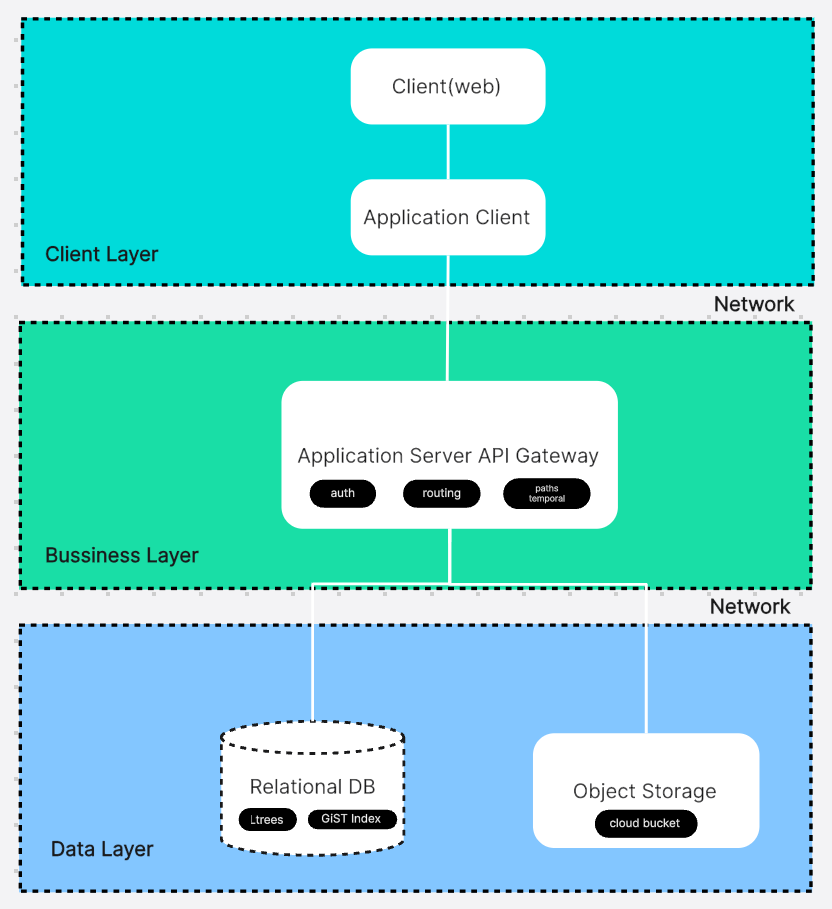
\includegraphics[width=\linewidth,height=0.4\textheight,keepaspectratio]{initialdbarch/architecture_diagram.png}
    \caption{Architecture High Level Model for the File Storage Platform.}
    \label{fig:architecture_diagram}
\end{figure}
\subsection{Entity Relationship Diagram - First Version}
\begin{figure}[H]
    \centering
    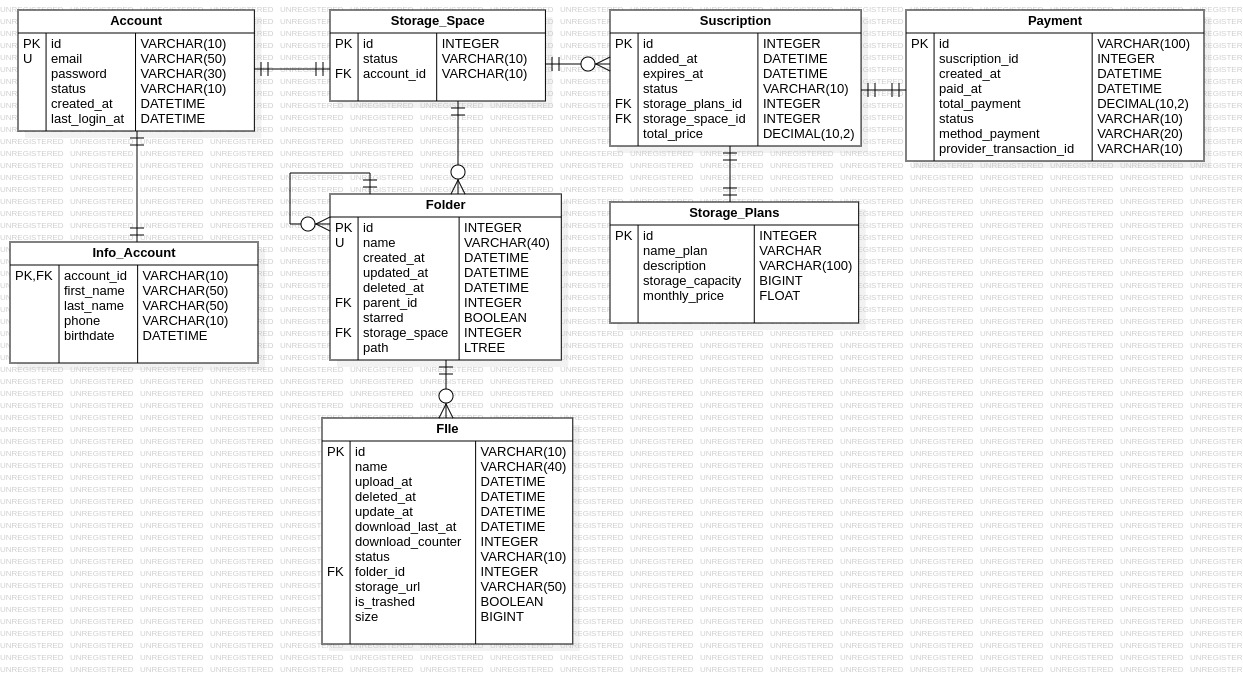
\includegraphics[width=\linewidth,height=0.95\textheight,keepaspectratio]{initialdbarch/ER.cloud.jpg}
    \caption{ First version of the entity relationship diagram for the file storage platform.}
    \label{fig:Entity Relaction}
\end{figure}
\subsubsection{Description of entities}
\begin{itemize}
    \item The \textbf{Account} entity represents the user account within the system. It contains main fields such as \textit{id}, \textit{email}, \textit{password}, \textit{status}, \textit{created\_at}, and \textit{last\_access}. Its role is to be the starting point for all user information, since both personal settings and storage space are derived from it.

    \item \textbf{Info\_Account} complements the account with personal data: \textit{first\_name}, \textit{last\_name}, \textit{phone}, and \textit{birthdate}. It is directly associated with Account and serves to store user identification information.

    \item The \textbf{Storage\_Space} entity manages the storage space allocated to each account. It includes \textit{id}, \textit{status}, and a foreign key \textit{account\_id}. Its role is to serve as a link between the user and their storage subscriptions.

    \item \textbf{Subscription} stores the data for an active subscription: \textit{id}, \textit{added\_at}, \textit{expires\_at}, \textit{status}, \textit{total\_price}, along with references to the contracted plan and storage space. Its function is to record the conditions of use of the service for a given period.

    \item The \textbf{Payment} entity represents the payments made for a subscription. It contains \textit{id}, \textit{created\_at}, \textit{paid\_at}, \textit{total\_payment}, and \textit{method\_payment}. It allows you to keep track of the charges associated with each service contract.

    \item The \textbf{Folder} entity organizes files into hierarchies. Its most important fields are \textit{id}, \textit{name}, \textit{created\_at}, \textit{updated\_at}, \textit{deleted\_at}, \textit{parent\_id}, and \textit{starred}. It represents directories that can contain files and subfolders.

    \item \textbf{File} stores user file information. It includes \textit{id}, \textit{name}, \textit{created\_at}, \textit{deleted\_at}, \textit{download\_counter}, \textit{size}, and \textit{folder\_id}. It is responsible for representing the digital content within the folders.

    \item The \textbf{Format\_File} entity describes the file format. It contains \textit{name}, \textit{description}, and \textit{extension}. Its function is to identify the file type and its basic characteristics.

    \item Finally, \textbf{Metadata} complements the file with specific information such as \textit{mime\_type}, \textit{title}, \textit{author}, \textit{storage\_backend}, and \textit{complete\_metadata}. It serves to expand the technical and descriptive details of each file.
\end{itemize}
\subsubsection{Description of Relationships between Entities}
\begin{itemize}
    \item Account is related to Info\_Account, as each account has associated personal information.
    \item Account is linked to Storage\_Space, indicating the storage space allocated to each user.
    \item Storage\_Space is connected to Subscription, which defines the terms of the contracted service.
    \item Subscription is associated with Payment, which allows the payments for each subscription to be recorded.
    \item Folder is organized hierarchically by its parent\_id, and in turn contains multiple Files.
    \item File is related to Format\_File, to define the file type, and to Metadata, which expands its descriptive information.
\end{itemize}
\subsection{Data Flow and Storage Solutions}

Here describes the overall data flow of the platform and the adopted storage solutions. It explains how information moves through the system and how files and metadata are managed across different storage layers.

\begin{figure}[H]
    \centering
    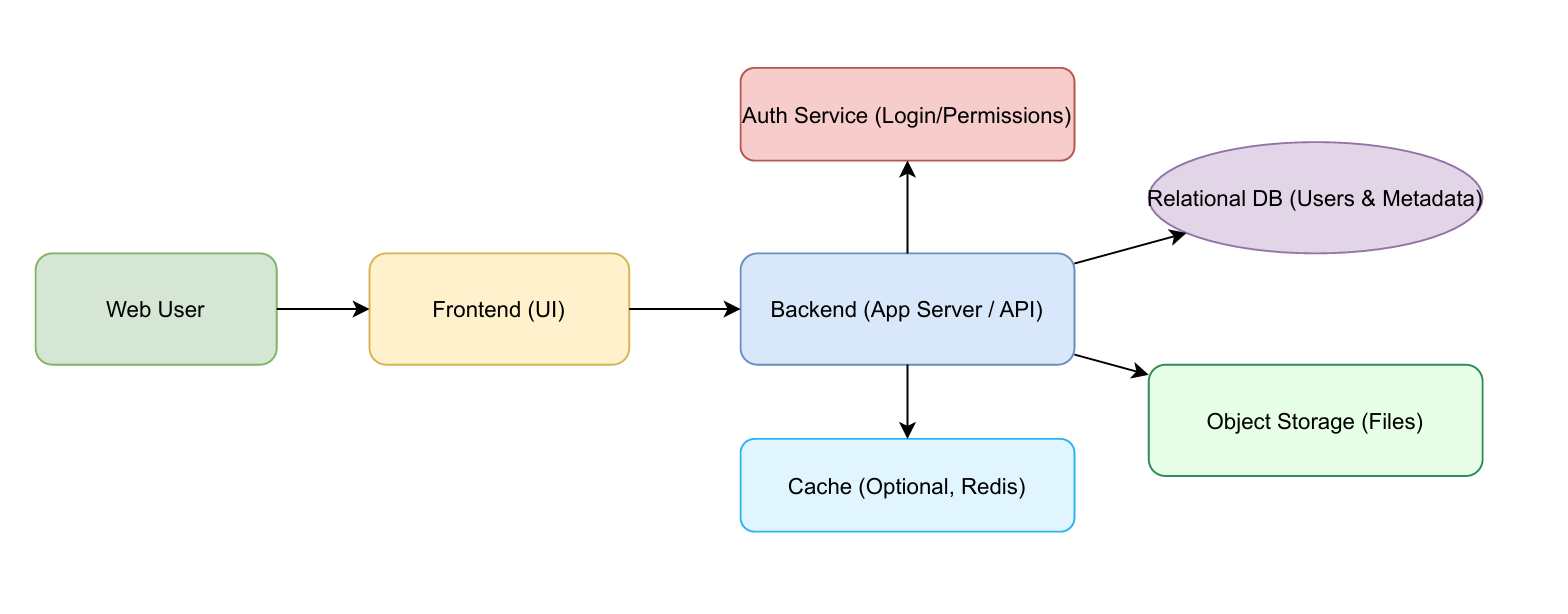
\includegraphics[width=0.95\linewidth,keepaspectratio]{initialdbarch/Dataflow.png}
    \caption{Data Flow and Storage Solutions for the file storage platform.}
    \label{fig:dataflow}
\end{figure}

For the dataflow, it proposed system manages two primary data types: user information and files. The data flow begins when a user interacts with the platform through the web or mobile interface. Requests are sent to the backend application server, which validates user credentials and permissions through the authentication service. Once authenticated, the backend processes the request according to its type:\\

\begin{itemize}
    \item For file uploads, the binary object is stored in the cloud object storage, while metadata, e.g., file name, size, type, upload date, and owner is recorded in the relational database.
    \item For file downloads, the backend verifies user access rights and generates a temporary signed URL, allowing secure file retrieval from the object storage.
    \item For queries such as listing files or browsing folders, the backend retrieves metadata from the database and may leverage a cache layer to accelerate frequent lookups.
\end{itemize}

This flow ensures that every operation is validated, traceable, and optimized for performance while maintaining strict access control. \\

Regarding storage solutions, its design adopts a hybrid model:

\begin{itemize}
    \item Relational Database: like PostgreSQL or MySQL is used for structured information such as user accounts, roles, permissions, and file metadata. This allows enforcing relationships and maintaining consistency.
    \item Object Storage: e.g., AWS S3, Azure Blob is used for binary files, ensuring scalability, durability, and redundancy. This approach allows efficient handling of large files with virtually unlimited capacity.
    \item Cache Layer: for supports faster access to frequently requested metadata, reducing database load.
    \item Backup and Replication strategies: ensure high availability and disaster recovery, minimizing the risk of data loss.
\end{itemize}

This architecture separates file storage from metadata management, providing scalability and flexibility. It also ensures that the platform can handle a growing number of users and files without compromising security, reliability, or performance.
